% $Id: introductionmbj.tex,v 1.3 1997/10/19 23:23:13 davek Exp davek $
\chapter{Introduction}\label{chap:intro}
This dissertation is concerned with the formal modelling and analysis
of embedded control systems. We adopt the view that the construction
and analysis of a formal model can contribute significantly to
increased confidence in correct system operation. Attention is
directed to distributed systems whose components communicate using a
broadcast communication network. The deployment of such systems is
becoming increasingly common, and ensuring the reliable fulfilment of
their intended function is a challenging problem. In the rest of
this chapter, the topics of embedded systems, formal methods and
broadcast communication are introduced. The chapter concludes with a
review of the approach and contribution of the dissertation.

\section{Embedded Control Systems}\label{sec:introembedded}
Embedded computer systems~\cite{kop:97} are pervasive in the
electronic equipment upon which we all are coming to
depend. Applications range from household products such as microwave
ovens, video recorders and cellular phones to control systems for the
transportation, chemical, electrical, gas, oil and nuclear
industries. What these computer systems have in common is that they
are \emph{embedded in a physical environment} with which they are
required to interact for the purpose of control or monitoring. The
role of the computer system in such interaction is typically
\begin{itemize}
\item to monitor significant variables of the environment such as temperature,
pressure, flow or level;  
\item to execute a control algorithm which takes as its input the values of 
environmental variables and compute output values in accordance with one or 
more mathematical models of the physical system;
\item to use values computed by the control algorithm to generate 
signals to the environment in order to control its function or optimise its 
performance.
\end{itemize}

The function of monitoring the environment is performed by physical
sensors within it. For example, a thermocouple produces an analogue signal (a
voltage) which varies with the temperature of the environment in which
it is placed. A digital value is obtained from an analogue signal by
A/D conversion, calibration and transformation to standard measurement
units (e.g. degrees Celsius) in a process known as \emph{signal
conditioning}. Such digital values are the inputs to the control algorithms
of the computer system.

Control algorithms are developed by control engineers who understand
the behaviour of the physical environment. The function of a control
algorithm is to generate output signals to the environment to influence
its behaviour so that some performance criterion is satisfied, even in
the presence of random disturbances.

Output from control algorithms is transmitted to the environment in
digital or analogue form.  For example, a digital output may cause a
heating element to be turned on or a valve to be closed, or an
analogue output, generated by a D/A converter, may vary a demand
voltage to an electric motor in order to control its speed.

Figure~\ref{fig:introflow} illustrates a simple embedded control
system~\cite{kop:97}. The objective of the control system is to maintain
the flow of liquid through a pipe at a set rate, despite changing
environmental conditions: varying level of liquid in the vessel or
temperature sensitive viscosity of the liquid, for example. The computer
interacts with its physical environment by monitoring the rate of
flow, using the flow sensor $F$, and adjusting the position of the control
valve to bring the flow rate as close as possible to the set-point. 

\begin{figure}
\centering
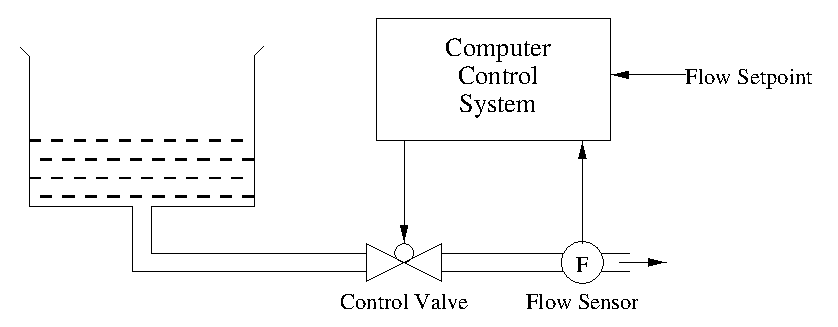
\includegraphics[width=.7\linewidth]{INTRO/flow.eps}
\caption{Simple Embedded Control System\label{fig:introflow}}
\end{figure}

In many systems, control is \emph{distributed} among several computing
nodes interconnected by a communication network~\cite{tor:98}. A
distributed computing system architecture is often a `good fit' with
the distributed nature of the physical environment. Cooperating
control units can be placed close to the physical devices which they
control, communicating with each other via a simple computer network
rather than the expensive and heavy wiring harness of traditional
control systems.  A distributed architecture also accords with sound
design principles such as modularity, dependability and 
scalability~\cite{kop:97}.

The emphasis in this work is on techniques for increasing confidence
in aspects of distributed system
\emph{dependability}. Laprie~\cite{lap:90} identifies dependability as
being concerned with those attributes of a computer system pertaining
to the quality of service which it delivers to its users over an
extended period of time. It is clear that failure of an embedded
system to deliver an acceptable quality of service may have
catastrophic consequences, either for the safety of the physical
environment or for the economic soundness of the system's supplier,
which may suffer as a result of the need to recall or repair many
faulty units of a mass produced commodity.

A crucial aspect of the dependability of an embedded system is its
ability to react to stimuli from the environment in a timely
way. More precisely, an embedded control system is a
\emph{real-time} system whose correctness depends not only on the
logical results of computations, but also on the physical instants at
which those results are produced~\cite{sta:88a}.  Real-time systems
are classified as either \emph{hard} or \emph{soft}. A
\emph{hard real-time system} is a real-time system in which a single
failure to produce a correct result within a specified interval of
time is regarded as unacceptable. A \emph{soft real-time system} is
one in which a (usually small) number of such failures, over a given
period of time, can be tolerated.
  
In this dissertation, we treat hard real-time systems, and are
particularly concerned with techniques which seek to contribute to the
assurance of system dependability by demonstrating that temporal
requirements are satisfied under all possible workloads. Such
techniques rely upon the \emph{predictability} of the temporal
properties of all aspects of system behaviour, including worst case
execution times of application code and operating system services, and
also communication latencies and hardware
performance~\cite{cvg:98,hal:93,hs:91}. The requirement for
predictability demands simplicity in system design, and when
necessary, flexibility and resource utilisation are sacrificed by
adopting \emph{static structures} which can be analysed at design
time.

\section{Formal Methods}
Formal methods entail the use of mathematically based languages,
techniques and tools for developing and reasoning about computer
hardware and software. The mathematics required is usually \emph{discrete
mathematics}, incorporating ideas from set theory and logic. The use of
mathematics has an impact both on the \emph{descriptive} and on the 
\emph{analytical} tasks which are required in the development of a computer 
system. For example, a descriptive task, such as specifying a set of
requirements, can be accomplished precisely, concisely, and
unambiguously using a mathematical language. Similarly, an analytical
task, such as demonstrating that a program function correctly
implements a high-level design, can be discharged convincingly using a
mathematically rigorous argument.  The objectives in applying a formal
method are to achieve clarity and precision in description, and to
reduce reliance on human intuition and judgement in analysis, making
greater use of mathematical \emph{calculation}.

This broad framework allows for a variety of \emph{levels of formality} in
the application of formal methods within a project. The NASA
guidebook~\cite{nas:97} identifies the following:
\begin{enumerate}
\item Level 1 methods involve the use of notations and concepts derived from 
discrete mathematics in order to develop more precise requirements
statements. Analysis, if any, is informal. There are no mechanical
tools (computerised algorithms) to support the writing or analysis of formal
expressions.
\item Level 2 methods involve the use of formalised specification languages 
with mechanised support tools ranging from syntax checkers and
pretty-printers to type checkers, interpreters and animators. Usually,
tool support for eliciting or checking mathematical arguments is not
available.
\item Level 3 methods involve the use of formal languages with rigorous 
semantics and correspondingly formal methods of semantical analysis
which support mechanisation.
\end{enumerate}
Wolper~\cite{wol:97} categorises methods at levels 1 and 2 as `weak'
formal methods and methods at level 3 as `strong'. His opinion is that
\begin{quote}
Without semantical analysis formal methods are of limited value with 
respect to their stated goal of ensuring the correctness of software
systems: their formal syntax and semantics are just theoretical properties,
not assets that are exploited in a substantial way. From the point of view of 
the author, a strong formal method even with limited applicability is more 
meaningful than a weak one that is perfectly general.
\end{quote}  

There is a similar latitude in the \emph{scope of application} of
formal methods within a project. For example, some stages in the
development life cycle may be singled out for particular attention,
certain system components may be identified as critical to mission
success or safety, and some system properties may be judged
particularly important and worthy of special attention.

Careful decisions are needed about the appropriate level of formality
and scope of application for each individual project, so that a good
balance can be achieved between the costs and benefits of formalisation.

In this work, we consider the problem of constructing formal models of
distributed embedded control systems, and of providing mechanical
assistance for the analysis of their functional and temporal
properties.  So the focus is on `strong' formal methods, in Wolper's
sense. As to scope of application, it is often acknowledged that a
formal model is useful in the design stages of a computer system, as
it facilitates the early detection of bugs and helps to avoid
expensive implementation of a faulty design. This is certainly the
case. In addition, however, we wish to emphasise the usefulness, for
embedded systems particularly, of a formal model of (some features of)
the implementation. The satisfaction of temporal properties of the
system usually depends crucially on implementation decisions whose
details may not be available in the early stages of design.  For
example, choice of processors and communication mechanisms, task and
message allocation and priorities, scheduling policies, and so on, can
all have a significant effect on real-time performance. It is
important to take steps to gain assurance that temporal requirements
which are satisfied by the design are also preserved in the implementation.

Experience suggests that successful application of formal methods in
an industrial setting depends upon a number of factors, including
\begin{itemize}
\item the use of expressive languages which are accessible to system
designers, being `intuitive' and `easy to use';
\item the availability of computer-based tools which provide prompt and 
useful feedback to their users; and
\item the ability to integrate the formal method into a familiar development
methodology, so that the method augments, rather than replaces,
traditional techniques.
\end{itemize} 

Many prominent formal methods are very expressive within a given
context: e.g., Z~\cite{spi:88} and VDM~\cite{jon:90} offer the full
generality of set theory and predicate calculus; Petri
nets~\cite{mur:89} offer a general model of concurrency, and Hybrid
Automata~\cite{hen:96} allow the expression of a wide variety of timed
systems. However, there is a growing interest in \emph{domain
specific} languages~\cite{jw:96}, which sacrifice generality of
expression in order to offer the system designer a more familiar
syntax, a greater ease of expression for typical applications within
their domain, and the possibility of tractable analysis supported by
software tools. It is hoped that these advantages can weaken resistance to 
the application of formal methods in industry by reducing the cost of 
model building and analysis. This is the approach followed here.

The need for automation and the provision of useful feedback to the user
has led to the increasing popularity of a style of analysis known as
\emph{model checking}~\cite{cgp:99}. Model checking is a technique which
relies on building a finite state transition model of a system and
checking that a desired property holds in that model. The basic
procedure in model checking is exhaustive state space search, which is
guaranteed to terminate since the model is finite. Once the model has
been constructed and the property of interest specified, the checking
is entirely automatic.  Furthermore, in the case that the property
does not hold in the model, a counterexample is generated, which can
provide the designer with valuable insight into the behaviour of the
system and aid in debugging.

The main obstacle in the application of model checking to industrial
scale systems is the size of the state spaces which arise in
exhaustive search.  This is known as the \emph{state explosion
problem}. There are many techniques for attacking this
problem~(\Sec\ref{ss:mscstateexplosion}). Here, we mention the
importance of \emph{abstraction}~\cite{lgs:95}. An abstract model
omits detail from the system description. However, it retains
sufficient detail to preserve system properties of interest. In this
way, the size of the state space to be searched is reduced and useful
questions can be decided in practice. Some abstract models are
\emph{exact}, i.e., for all properties of interest, the property holds
for the model iff it holds for the system. Other abstract models are
\emph{conservative approximations}, i.e., if a property holds for the
model, it also holds for the system; but, if it does not hold for the
model, its status with respect to the system is undecided. Clearly, an
exact abstraction is desirable, but a conservative approximation may
lead to a greater reduction in the size of the state space. If a
property fails to hold in a conservative approximation, further
investigation is required to determine if the failure is a genuine
feature of the system, or an aberration caused by the approximation.
Conservative approximations have been used successfully to analyse the
behaviour of embedded system implementations~\cite{bhkr:94b,cor:96} and
they are used extensively in the rest of the dissertation. 

Even an abstract formal model can produce a state space which is
too large to search completely in a reasonable amount of time or
memory. Nevertheless, the model can be used effectively for
\emph{debugging} the design or implementation from which it is
derived. The focus here changes from verification based on exhaustive
search to \emph{falsification} based on semi-exhaustive
search~\cite{fkf:99}. Techniques motivated by this point of view
include state storage methods which allow a small probability that
some reachable states are not explored~\cite{hol:95,ste:97} and
simulation techniques which aim for a saturated coverage of the state
space~\cite{ga:98,ysa:97}. The coverage provided by these methods can improve
significantly on traditional validation techniques such as simulation
and testing~\cite{mye:79}.

In summary, formal methods are one important approach among several
for gaining increased confidence in system dependability. The benefits
include increased understanding gained from the
construction and analysis of formal models, improved communication
made possible by formal documentation, and a formal basis provided for
the construction of software tools to assist in system development.

\section{Broadcast Communication\label{sec:can}}
The communication architecture encountered most frequently in the
implementation of distributed embedded control systems is the 
\emph{broadcast bus}~\cite{uk:94}. In broadcast communication,
a message transmitted from a single sending node can be received
directly by all nodes connected to the network. This contrasts with
point-to-point communication in which messages are transmitted from a
single sender to a single receiver. The use of a broadcast bus
simplifies implementation of the common requirement in an embedded
system to provide a consistent view of the state of the physical
environment to a number of different nodes, e.g., to a man-machine
interface, a process control node and an alarm-monitoring
node~\cite{kop:97}. It can also simplify the implementation of clock
synchronisation and the tolerance of individual node failures.

A wide variety of broadcast protocols is seen in practice, each
offering a solution to the problems posed by a particular application
area, e.g., Profibus~\cite{din:89} for process control,
LON~\cite{ech:91} for building automation and CAN~\cite{iso:11898},
TTP~\cite{kop:93} and QWIK~\cite{jo:99} for automotive applications.
It is not our intention to review this extensive field here. Surveys
of the relevant principles and applications can be found
in~\cite{kop:97,ks:97,uk:94,ver:97b}. However, we do offer a more
detailed consideration of one such protocol, CAN, which is the basis
of the formal model presented later in the dissertation and will serve
as our canonical example of broadcast communication.

\subsection{Controller Area Network}
Controller Area Network (CAN)~\cite{bos:91,iso:11898} is a simple,
deterministic, broadcast communication protocol which is not only
attractive to system developers but also amenable to formal modelling
and analysis. It is gaining increasing importance and attention in the
implementation of distributed real-time systems, as evidenced by the
variety of contributions in the proceedings of recent International
CAN Conferences~\cite{cia:99}.

CAN provides multi-master, priority-based bus access using a CSMA/CD
protocol similar to Ethernet's, but with a deterministic collision
resolution policy which makes it suitable for use in hard real-time
systems.  It is a robust protocol offering high reliability even in
harsh electromagnetic environments and is suitable for the
transmission of short messages over a small area at speeds of up to
1~Mbit/s.  CAN was developed by Bosch in the mid-eighties in order to
reduce the need for complex wiring harnesses in the automotive
industry.  Its use in the European car industry has grown to the point
where it is an acknowledged industry standard and its popularity is
growing in the USA where it has been accepted as a standard by the SAE
for bus and truck manufacture~\cite{sae:92}. The availability of low
cost components from a variety of manufacturers, who are seeking to
satisfy the high volume requirements of the automotive industry, has
encouraged the use of CAN in an expanding range of application areas,
including: medical, packaging control, agricultural machinery, lift
control, measurement, robot control and PLC controlled manufacturing.

\subsubsection{CAN Operation}
Information is transmitted as fixed format {\em frames\/} which consist of a
\emph{message identifier}, 0 to 8 \emph{data bytes} and sundry \emph{control}
bits as shown in figure~\ref{fig:canframe}. The physical medium is
usually twisted pair cable over which frames are transmitted using NRZ
encoding with stuff bits inserted when needed to preserve
synchronisation.  When the bus is idle, any connected node may start
to transmit a new frame.  If two or more nodes start to transmit
frames at the same time, the bus access conflict is resolved by
non-destructive bitwise arbitration which is based upon the message
identifier. The bitwise arbitration mechanism classifies bits as either
\emph{dominant} or \emph{recessive}. During transmission of the arbitration
field, transmitting nodes monitor the bus. Transmission of a dominant
bit by any node causes all nodes to monitor a dominant bit on the bus;
only if all transmitting nodes send a recessive bit is the monitored
bit recessive. If the transmitted bit is recessive, but a dominant bit
is detected on the bus, the transmitting node recognises that it has
lost the bus arbitration, ceases transmission of its frame and behaves
as a receiver of the highest priority competing frame. In a standard
CAN frame, the arbitration field consists of the message identifier
and the RTR (Remote-Transmit-Request) bit. A message identifier
consists of 11 (29) bits in the standard (extended) frame format and
is interpreted as a non-negative integer assigning a priority to the
frame. Priorities are assigned in monotonically decreasing order
starting from 0. The transmitter with the frame of highest priority
gains bus access {\em without\/} experiencing any delay due to the
access conflict, i.e. it behaves as if it were the only node seeking
access to the bus. This property makes the bus particularly suitable
for predictable, real-time communication. Frames which are disturbed
either by losing arbitration or by the occurrence of errors during
transmission are retransmitted automatically when the bus becomes idle
again.  A frame which is retransmitted is handled like any other
frame, i.e.  it participates again in the arbitration process in order
to gain bus access.

In addition to giving a priority to a frame, the message identifier is also
used by each receiving node to determine whether or not it wishes to `accept'
the frame. There is no address associated with a frame to indicate its
intended recipient. Each node connected to the bus performs an acceptance
test during, or shortly after, the transmission of a frame. If the frame
passes the test, its data field is made available to the accepting node,
otherwise the node ignores the frame.

\begin{figure}
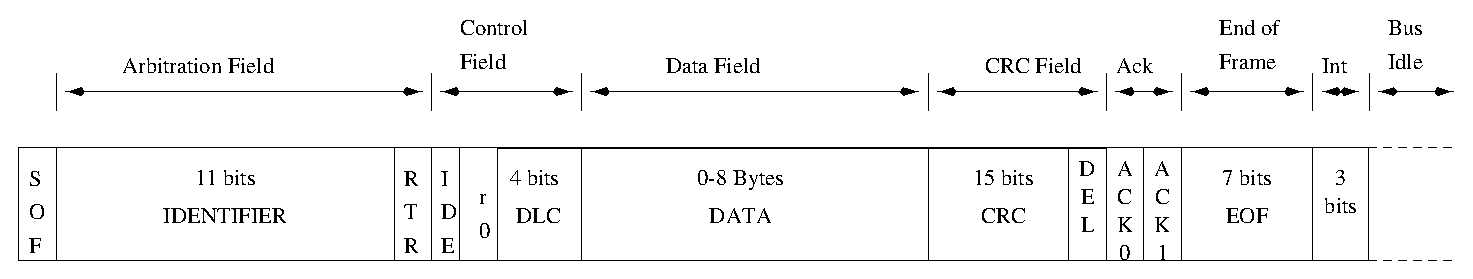
\includegraphics[width=\linewidth]{INTRO/canframe.eps}
\caption{CAN Frame -- Standard Format\label{fig:canframe}}
\end{figure}

\subsubsection{CAN-based protocols and analysis}
There has been much interest in developing CAN-based protocols and
analysis to solve a variety of typical distributed system problems.
Tindell~et~al.~\cite{thw:94} show how fixed priority pre-emptive
scheduling analysis can be applied in order to bound message response time for
systems with a suitably restricted computational model~\cite{tbw:95}.
Another approach to message scheduling is presented in~\cite{lkj:99},
in which hard real-time messages are allocated off-line to slots in a
Time Division Multiple Access (TDMA) schedule~\cite{ks:97}, with
redundant time slots provided to achieve some fault tolerance; the
redundant slots are used in the Earliest Deadline First (EDF)
scheduling~\cite{ks:97} of soft real-time messages, in the case of
error-free transmission. Ver{\'\i}ssimo~et~al.~\cite{vrm:97} derive
bounds for bus inaccessibility under a variety of fault
scenarios. Protocols for achieving atomic broadcast in the presence of
network faults are given in~\cite{rva:98} and~\cite{lk:99}. A solution
to the problem of fault-tolerant clock synchronisation is presented
in~\cite{rgr:98}.  The only other formal study of CAN-based
communication, so far as we know, is the Z specification of the
protocol by Benzekri and Bruel~\cite{bb:97}; however, real-time and
performance aspects are not discussed in their work.

\section{The dissertation}
\subsection{Justification}
The work presented in this dissertation addresses the problem of
providing a \emph{high-level language} for modelling embedded systems
which communicate using \emph{broadcast communication}, with a view to
exploiting \emph{efficient, automated analysis techniques} in order to
increase confidence in the satisfaction of temporal system properties.
We briefly justify our belief in the need for work in these areas.
\begin{description}
\item[High-level language]  
We have argued that a formal approach to system development is an
important component in the construction of dependable systems, and
that high-level languages and computer-aided analysis are required if
formal methods are to be of practical use in industry. Much recent
research on formal analysis of real-time systems has concentrated on
techniques based on timed automata~\cite{ad:90}. However, the language
of timed automata is generally acknowledged to be too low-level for
general use~\cite{ad:94,bfk:98,tri:98,pet:99}.  Therefore, there is a
need for research on methods to exploit the analysis techniques
developed for timed automata in the context of high-level languages
for modelling and development.

\item[Broadcast communication]
An increasing number of distributed embedded systems are implemented
which rely on broadcast communication.  CAN is a simple, predictable
broadcast protocol which is coming to dominate a large sector of this
market. As it is often employed in systems which demand high
dependability, there is considerable interest in the question of how
to apply formal methods in the development of CAN-based
systems. Currently available methods, however, do not offer a
straightforward way to model systems which communicate via the CAN protocol.
Our work is aimed at providing such a method.

\item[Efficient analysis]
A high-level language for modelling broadcast systems will only be
useful in so far as there are efficient techniques for analysing
the models which are described with it. Our work shows how existing
techniques can be applied and also proposes new techniques for efficient
analysis.   
\end{description}

\subsection{Structure and contribution}
Chapter~\ref{chap:methods} introduces labelled timed transition
systems as a basic model for real-time systems and describes how
such models can be derived using either timed automata or timed
process algebra.  The use of automata and temporal logic for
the specification of system properties is presented. Techniques for 
verifying that a timed model possesses specified properties are
described in some detail. This chapter presents no new results but is the
foundation on which the rest of the dissertation is built. 
 
Chapter~\ref{chap:bcandle} presents a new system modelling language,
called \bcandle, which allows the expression of process behaviour using a
small set of process operators, includes primitives for broadcast
communication based on a CAN-style protocol, and permits the modelling
of both data and control structures. It is shown that the language
satisfies a number of algebraic laws and is expressive enough to model
essential features of CAN communication, including message priorities
and channel latency, as well as standard real-time constructs, such as
timeouts and watchdog timers. So far as we know, this is the first
formally defined language which treats broadcast communication with 
prioritised message passing over latent channels in a dense time 
framework.

Chapter~\ref{chap:tggen} defines a translation to timed automata for a
large subset of \bcandle\ systems. An efficient method for
performing the translation is described and implemented. This work
builds upon and extends the approach developed by Garavel in the
translation of LOTOS~\cite{gar:92} and of Yovine in the translation of
ATP~\cite{yov:93}. We demonstrate the use of the method by applying it
to a simple \bcandle\ model which is analysed using the
KRONOS~\cite{bdm:98} model-checking tool.

Chapter~\ref{chap:sggen} presents two techniques for efficient analysis
of \bcandle\ models: firstly, an on-the-fly generation of the
simulation graph, incorporating clock activity reduction; secondly, a
BDD-like, compact representation of the state space which treats discrete
data variables and clock variables in a uniform manner. The application 
of the latter technique to timed systems is entirely novel. The former
technique is based upon a combination of methods which is presented here
for the first time.  

Chapter~\ref{chap:practice} serves to validate the ideas 
presented in Chapters~\ref{chap:bcandle}--\ref{chap:sggen}, and to
point the way to future developments. It presents a high-level
modelling language whose semantics are given by translation to
\bcandle, so providing a route to the use of the numerous analysis 
techniques based on timed automata, including those introduced in
Chapter~\ref{chap:sggen}. The framework
of a practical modelling and analysis environment is outlined. The
utility and limitations of the techniques are illustrated in a small
case study.

Chapter~\ref{chap:conc} summarises the work and suggests lines of
future enquiry. Related work is referred to and discussed in context.












